\documentclass[preprint2,epsf,epsfig,graphics]{emulateapj}
\usepackage[draft]{hyperref}
\usepackage{graphicx}
\usepackage{color}
\usepackage{natbib}
\shorttitle{The SGP at 145\,MHz with PAPER}
\shortauthors{Kohn et al.}

\newcommand {\aplt} {\ {\raise-.5ex\hbox{$\buildrel<\over\sim$}}\ }

\begin{document}

\title{Measurements of the Southern Galactic Plane at 145\,MHz with PAPER}

\author{Saul A. Kohn\altaffilmark{1,$\dagger$}}
\author{James E. Aguirre\altaffilmark{1,$\dagger$}}
\author{Will Saunders\altaffilmark{1,$\dagger$}}
\author{Aaron Parsons\altaffilmark{2,3}}
\author{et al.\altaffilmark{4}}

\email{saulkohn@sas.upenn.edu (corresponding author)}

\altaffiltext{1}{Department of Physics and Astronomy, University of Pennsylvania, Philadelphia, PA 19104}
\altaffiltext{$\dagger$}{These authors contributed equally to this work.}
\altaffiltext{2}{Astronomy Dept., U. California, Berkeley CA}
\altaffiltext{3}{Radio Astronomy Lab., U. California, Berkeley CA}
\altaffiltext{4}{a lot of other places}

\begin{abstract}
Present astrophysical understanding of high-mass stars allows for predictions of their formation rates.  High-mass stars explode in supernovae, which leave behind Supernova Remnants (SNRs) that serve as records of the stars; however the $\sim$300 observed SNRs is far fewer than the $>1000$ predicted.  This gap could implicate the understanding of high-mass stars if confirmed. 
Meanwhile, there is presently a dearth of low-frequency radio measurements ($\nu\aplt$200\,MHz) of sources in the Southern Galactic Plane (SGP).
This study reports on a search for SNRs as well as measurements of sources in the SGP using low-frequency radio maps produced at 145\,MHz by Precision Array for Probing the Epoch of Reionization (PAPER).
{\color{red} VERY BRIEF SUMMARY OF FINDINGS.}
{\color{blue} CAN WE ARGUE FOR GOOD POINTS OF LOW-RES?}
%Mathematical predictions {\color{red}[CITE!!]} of the number of observable SNRs based on known limitations showed that the SNR Defect may be made up by a complete survey.  This shows that the SNR Defect is likely due to selection effects: difficulties in detecting SNRs given their location and size, and not due to a fundamental misunderstanding in star formation rates.
\end{abstract}
\keywords{ISM: - molecular clouds -- stars: formation}

\section{Introduction}

The major classification difference between high-mass ($M > 8M_{\odot}$ ) and low-mass ($M < 8 M_\odot$) stars is the end of their life, for which the latter explode in supernovae (SNe), which is precipitated by accumulated inert iron in the core \citep{Arnett.73}.  
The subsequent collapse of the core creates the supernova explosion, which ejects the entirety of the star’s outer layers, forming a supernova remnant (SNR).  The SNR consists of the expanding supernova shock wave, the ejected outer material of the star, and any dust or gas it picks up while expanding.  
The remnant slowly expands until its density becomes near that of the surrounding interstellar medium (ISM) making it effectively indistinguishable, and ending its existence as an SNR.  
The SNR shock releases high-velocity particles, including a barrage of electrons that produce non-thermal emissions; these relativistic electrons are accelerated and spiraled by the magnetic fields of the SNR and produce synchrotron radiation as a result making SNRs easily-detectable radio sources \citep[e.g.][]{Burbidge.56,Stupar_cat.11}. 
Since SNRs are relatively short-lived ($\sim10^5$ yr), which means that they can serve as a record of recent star formation rates of high-mass stars, since stars of high mass has shorter lifetimes {\color{red}[CITE!!!]}.  
Therefore by counting remnants, one can expect to learn about recent star formation {\color{red}[messy phrasing]}.
Measuring the star formation rates through iron abundance allows for a reasonable prediction of the number of galactic SNRs; however, these predictions imply that there should be far more SNRs than currently detected \citep[e.g.][]{Brogan.06}.  

%Supernovae are classified according to spectral features into two types: Type I have no hydrogen in their spectra while Type II have hydrogen present; furthermore, Type I are classified into Ia, which are actually white dwarf supernovae, not stellar supernovae, Ib, which contain helium in their spectra, and Ic, which do not contain helium \citep{mms13}.
%{\color{red}[DOES THIS CONTRIBUTE TO THE OVERALL PAPER?]}
%SNRs are categorized, based on their morphology, into two traditional classes: 
%\begin{itemize}
%\item[(i)] shell-like, which have a complete shell resulting from the SNR shock;
%\item[(ii)] plerionic or ``crab-type,'' which have centrally located pulsars, also known as plerions, \citep{Weiler_crab.78}
%\end{itemize} 
%Recent observations {\color{red}[CITE!!!]} have extended the classification system to include: 
%\begin{itemize}
%\item[(iii)] composite, which may contain both a shell or partial shell and central pulsar; and
%\item[(iv)] mixed-morphology, which contain a combination of standard SNR features and unusual characteristics including non-ejecta material and/or interactions with molecular or HI clouds \citep{Rho.98}
%\end{itemize}


To date, 294 SNRs have been catalogued \citep{DAGreen.14} despite the prediction based on the Galactic star formation rate that $\sim10^3$ galactic SNRs exist \citep{Li.91}.  
Assuming a rate of two SNe per century, $\sim2000$ SNRs are predicted in the galaxy \citep{Pavlovic.13}.  
Additionally, \cite{Brogan.06}, were able to make assumptions based on known limitations of VLA surveys in order to predict the number of SNRs that are observable at all. {\color{red}[What were the assumptions?]}
Their study yielded a result of 460 observable SNRs {\color{red}[I don't understand this -- why 460, rather than 294?]}; this is still less than half of the observed value, which leaves many SNRs unaccounted for. 
This “SNR Defect” has thus far been attributed to selection effects, a general grouping of difficulties in observing SNRs that includes: 
\begin{itemize}
\item[(i)] SNRs occur in dusty regions, where the dust may absorb and/or deflect SNR emissions traveling toward earth;
\item[(ii)] since the vast majority of stars are located along the galactic plane, so are most SNRs, increasing potential source confusion \citep[e.g.][]{Gao_v.11,Gao_vi.11};
\item[(iii)] due to the inverse square law of observed luminosity, doubling the distance to an object reduces its apparent brightness by one-fourth  \citep{Green.91}. The light from SNRs located 50,000 ly away, for example, is diminished by a factor of $\sim$300;
\item[(iv)] superpositioning along the Earth’s line of sight, by which nearby, young  and inherently dense SNRs block or severely inhibit the entire field of view behind them, making surveys of the SNR population more difficult {\color{red}[CITE?]}. 
\end{itemize}
{\color{red}[NOW WE NEED TO SAY SOMETHING ABOUT HOW LOW-FREQ CAN HELP WITH THIS?]}

It has long been known {\color{red}[CITE!!!]} that some larger SNRs, such as W28 and W30 {\color{red}[GIVE POSITIONS]}, have positioned within them \ion{H}{2} regions and other sources of thermal emissions, which increase the likelihood of misidentification \citep{Andrews.85}.  \cite{Brogan.06} showed that the small likelihood of actual proximity notwithstanding, the apparent proximity interferes with detection of SNRs.  As a result, much has been invested in finding a method to mitigate the selection effects. 

Radio surveys have typically been used to observe shell-like SNRs %and are successful 
because of the emission spectra and morphology of those SNRs \citep{Bandiera.01}.  {\color{red}[NEEDS MORE EXPLANATION -- this is a conference talk, we should cite a resultant publication]}

Young SNRs, which are compact and have close-to-blackbody emission spectra are more easily detected by high-resolution {\color{red}[WAVELENGTH?]} surveys, whereas older SNRs, which are more diffuse and emit mostly low frequencies, are better detected with radio surveys {\color{red}[CITE!!!]}. \cite{Stupar_cat.11} searched for H$\alpha$ emission coming from known SNRs in order to better identify specific structures {\color{red}[need more detail here]} within the remnants with greater resolution than radio or optical.  Recent X-ray surveys {\color{red}[CITE!!!]} have also been successful in observing SNRs, but usually require supplemental information due to known limitations {\color{red}[for example...?]} \citep{Bandiera.01}. While observing at radio frequencies mitigates most of the confusion when observing the Galactic plane {\color{red}[how true is this?]}, \ion{H}{2} regions pose a more significant problem.  \ion{H}{2} regions, opposed to SNRs, thermally emit from heating causing by a nearby high-mass stars (usually main-sequence O or B).  Recent discoveries {\color{red}[CITE!!!]} that some SNRs were actually galactic \ion{H}{2} regions have increased the push for surveys to better differentiate them {\color{red}[for example (survey, rather than single one below)?]}.  For example, SNR G166.2+2.5 was discovered to be an \ion{H}{2} region heated by O7.5V star BD+41 1144 \citep{Foster.06}.  

The Southern Galactic Plane (SGP) has been measured at various radio frequencies, including the Molonglo Galactic Plane Survey \citep[MGPS][]{Murphy.07} and the Molonglo Observatory Synthesis Telescope SNR Catalog \citep[MOSTSNRCAT][]{Whiteoak.96} at 843\,MHz, the synthetic catalogs of SNRs at 1\,GHz \citep{DAGreen.14} and \ion{H}{2} regions at 2.7\,GHz \citep{Paladini.03}. {\color{red} I don't like this paragraph, but it'll do for now.} Infrared measurements of the SGP were made by, e.g., the Midcourse Space Experiment \citep[MSX][operating at 8.28--21.3\,$\mu$m (36.23--14.08\,THz)]{Egan.03}. However, there is a dearth of measurements of the SGP at very low radio frequencies ($\nu\aplt$200\,MHz).

This work presents measurements of sources in the SGP using the Precision Array for Probing the Epoch of Reionization (PAPER), a low-frequency radio telescope that observes at a central frequency of 145\,MHz. The paper is laid out as follows. In section~\ref{sec:obs} we discuss the acquisition and reduction of PAPER's measurements of the SGP. Section~\ref{sec:res} presents our map of the SGP, with detections of SNRs, \ion{H}{2} regions and extragalactic sources cross-matched with the many of the catalogs listed above. We investigate those sources which do not match with any of the catalogs. In Section~\ref{sec:disc} we {\color{red} DISCUSS THINGS}. We summarize and conclude our study in Section~\ref{sec:conc}, with an eye towards future imaging surveys with PAPER and its successor, the Hydrogen Epoch of Reionization Array (HERA).

\section{Observations}
\label{sec:obs}

The Precision Array for Probing the Epoch of Reionization (PAPER) is an experiment designed to set the strongest limits on, and possibly detect, the 21\,cm signal of neutral hydrogen at redshifts $z \geq 7.5$. It is operated in the Karoo, South Africa (-30:43:17.5 N, 21:25:41.9 E). To be able to set the strong limits it has to date \citep[][Cheng et al. in prep., Kohn et al. in prep.?]{Parsons.14, Jacobs.14, Ali.15, Moore.15}, it requires a highly redundant configuration to maximise its sensitivity to a few discrete uvw voxels \citep[e.g.][]{Parsons.12}. However, in July and September 2011 the array was briefly reconfigured into an imaging array in order to do image-based analysis of the low-frequency radio sky \citep[e.g.][]{Stefan.13}. The imaging configuration and its instantaneous uv coverage is shown in Figure~\ref{fig:config}.

\begin{figure}
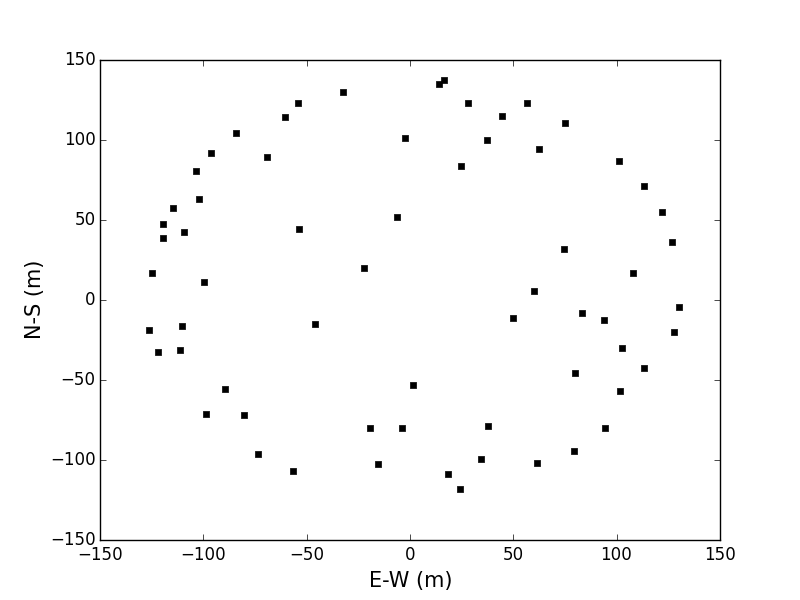
\includegraphics[width=\columnwidth]{psa64imageconfig.png}
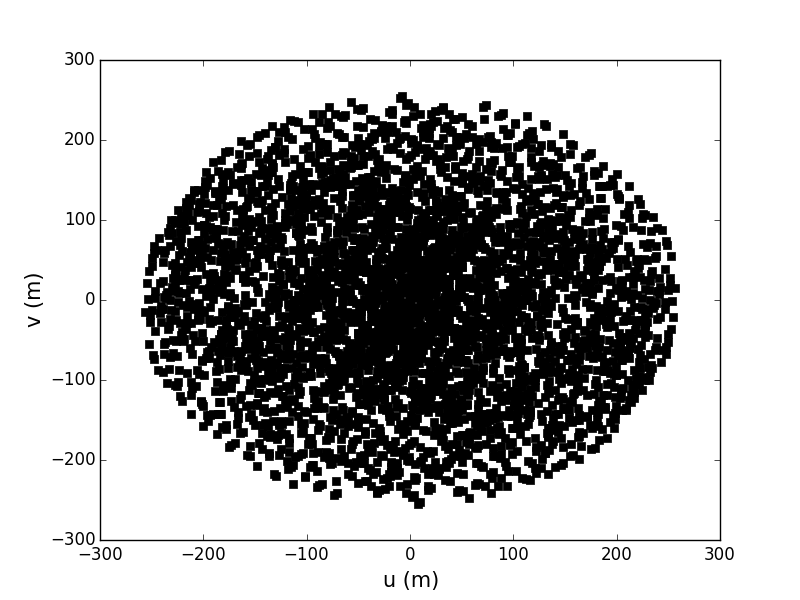
\includegraphics[width=\columnwidth]{psa64uvcoverage.png}
\caption{\textit{Above}: The PAPER-64 single-polarization configuration that took the measurements we report on in this paper. The antennae were arranged in a pseudo-random scatter in order to optimize uv-coverage. \textit{Below}: The resultant instantaneous uv-coverage. Maximum voxel occupancy is $\sim70$.}
\label{fig:config}
\end{figure}

In this work we present measurements made overnight July 4--5th 2011.
{\color{blue}[JEA] $\rightarrow$}Map details: DECONVOLUTION, (CALIBRATION?), zenith, FoV, cuts made etc.

\section{Results}
\label{sec:res}

Our map of the SGP is shown in Figure~{\color{red}[NUMBER]... DETAILS}.

Source identification and extraction was performed using PyBDSM\footnote{\url{http://www.lofar.org/wiki/doku.php?id=public:user software:pybdsm}}, which identified all sources $\geq3\sigma$ above their local background, accounting for possible sidelobe confusion \citep{PyBDSM.15}. To each detected source we fit a two-dimensional, 20' FWHM Gaussian to approximate the PAPER beam \citep{Parsons.10} in order to extract the source flux. We detected $446$ {\color{red} [NOT QUITE UNIQUE -- NEED TO TIDY UP]} individual sources, the properties of which are shown in Table~{\color{red}[NUMBER]... DETAILS}. 

Mention Molonglo Reference Catalogue of Radio Sources \citep[MRC][]{Large.81} .

\begin{figure}
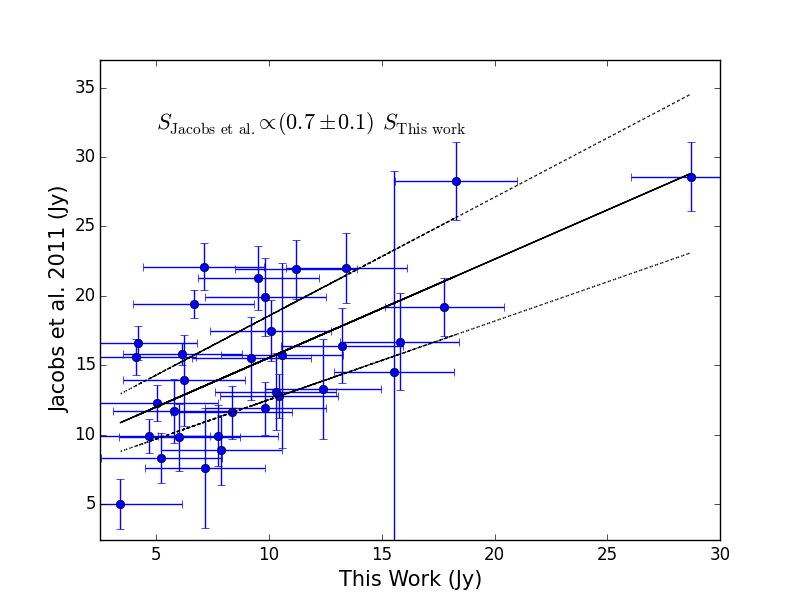
\includegraphics[width=\columnwidth]{us_and_danny_cal.png}
\caption{A comparison of the fluxes of extragalactic MRC sources measured by \cite{Jacobs.11} at 145\,MHz, compared to our own. The measurements are consistent to within 1$\sigma$. A line of best fit is shown (solid line) along with $\pm1\sigma$ on the best fit parameters (shaded region).}
\end{figure}

\begin{figure}
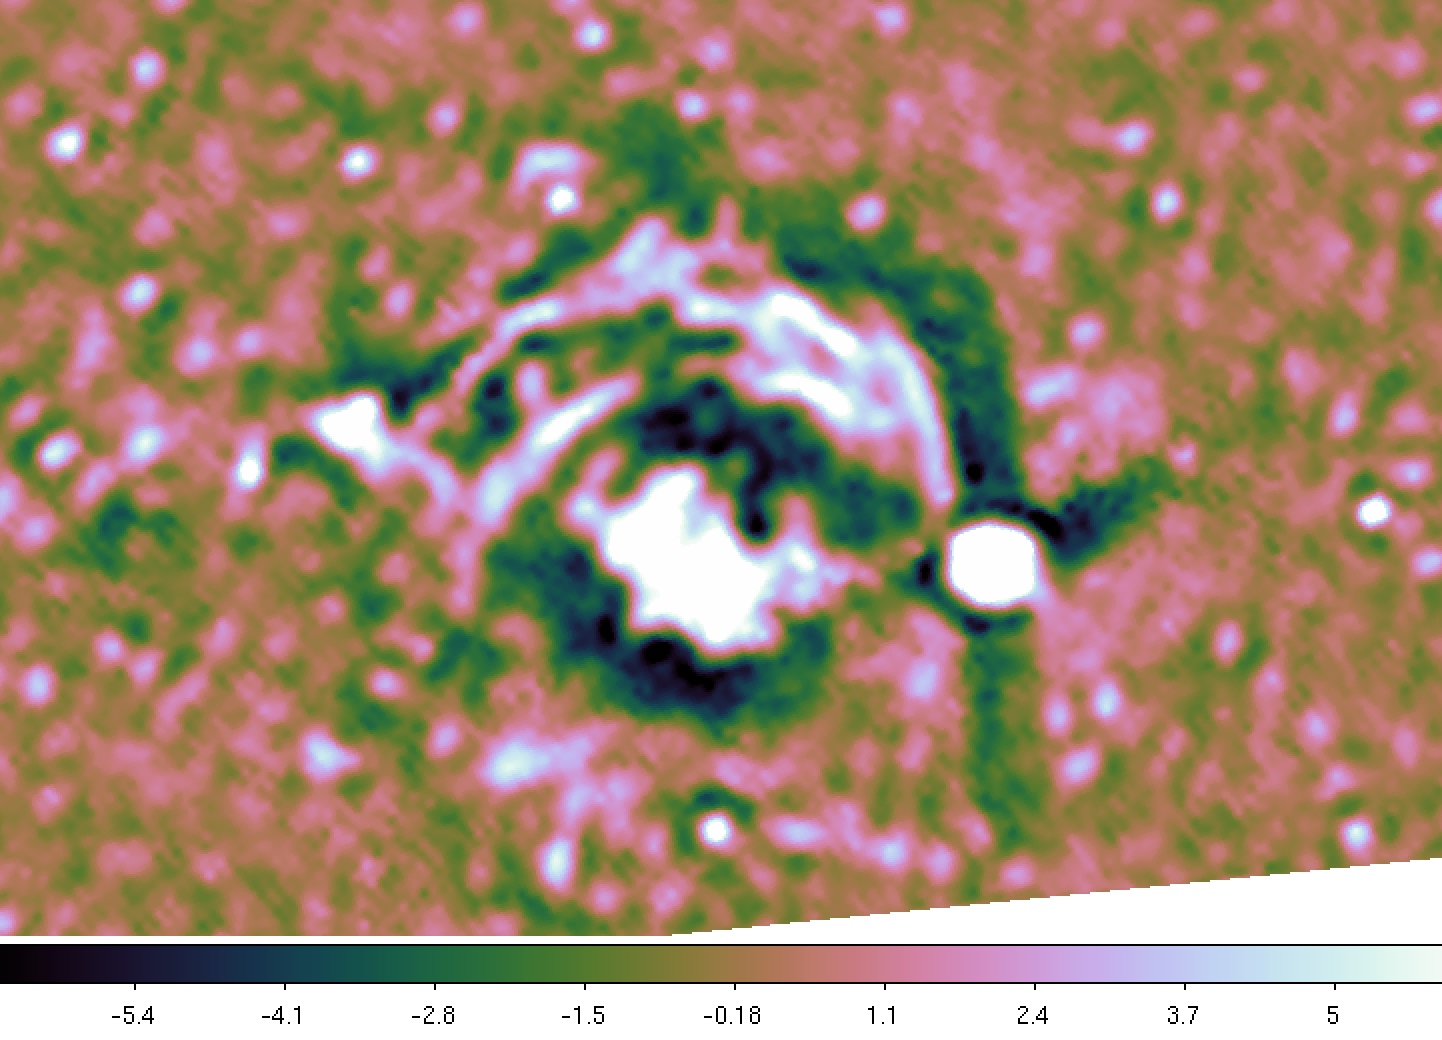
\includegraphics[width=\columnwidth]{vela_cubehelix.png}
\caption{The Vela and Puppis SNRs}
\end{figure}

\begin{itemize}
\item Figures:
\begin{itemize}
	\item countour map of SGP, overlaid with... something? Green, Paladini, MSCAT, etc. Could also have background image, if we want.
	\item more pretty pictures: zoom-in of an interesting region that looks to be nicely-cleaned, just our image, no contours [e.g. Vela]
\end{itemize}
\item Tables: 
	\begin{itemize}
	\item our sources -- Number, RA, Dec, 145\,MHz flux, Maj axis/radius(, surface brightness?)
	\item comparison to other catalogs:
		\begin{itemize}
		\item SNRs
		\item \ion{H}{2} regions
		\item galaxies
		\item others
		\end{itemize}
	\end{itemize}	
\item Graphs:
	\begin{itemize}
	\item Histograms of things?
	\end{itemize}
\item Spectral indices?
\end{itemize}


\section{Discussion}
\label{sec:disc}

\begin{itemize}
\item SNR defect
\item AOB
\end{itemize}

\section{Conclusions}
\label{sec:conc}

\begin{itemize}
\item Summarize findings
\item Brag about being the first low-freq measurements
\item Maybe brag about the maybe benefits of low-res measurements
\item Throw-out to polarized sky survey (Nunhokee et al. in prep.) and a future polarized galactic plane survey (Aguirre et al. in prep?).
\item Throw out to imaging capabilities of HERA\footnote{\url{www.reionization.org}}.
\end{itemize}

%\clearpage
\appendix

\section{Catalogs}

\begin{deluxetable}{cllll}
\tabletypesize{\scriptsize}
%\rotate
\tablecaption{Detected properties of sources in the SGP (abridged) \label{tab:PyBDSM}}
%
\tablewidth{0pt}
\tablehead{																					
\colhead{Source} & \colhead{RA} & \colhead{Dec} & \colhead{S$_{145}$} & \colhead{Semi-major axis}    \\
\colhead{Number}&\colhead{deg}&\colhead{deg}&\colhead{Jy}&\colhead{arcmin} 
} 		
\startdata                         
0 & 91.701652 & 8.6792533 & 4$\pm$2 & 22$\pm$6 \\
1 & 93.979553 & 9.3652856 & 10$\pm$2 & 39$\pm$18 \\
2 & 94.297523 & 9.8516745 & 8$\pm$2 & 27$\pm$8 \\
3 & 94.417152 & 8.6335312 & 10$\pm$2 & 32$\pm$9 \\
4 & 95.988954 & 10.269745 & 1$\pm$2 & 12$\pm$2 \\
5 & 96.505227 & 4.3765538 & 44$\pm$1 & 75$\pm$19 \\
6 & 97.007929 & 10.371556 & 5$\pm$2 & 21$\pm$4 \\
7 & 98.43141 & 11.608658 & 12$\pm$2 & 39$\pm$12 \\
8 & 98.551229 & 10.667595 & 0$\pm$1 & 5$\pm$0 \\
9 & 98.554268 & 10.396245 & 68$\pm$1 & 88$\pm$16 \\
10 & 98.808621 & 10.587542 & 1$\pm$1 & 8$\pm$0 \\
\enddata
\end{deluxetable}
\clearpage
\bibliographystyle{plainnat}
\bibliography{snrbib}{}

\end{document}